%-------------------------------------------------------------------------------
% ELIMINATIONS OF REDUNDANCY
%-------------------------------------------------------------------------------
\subsection{Reducing redundancy}
\begin{frame}{What FCA brings to the table}{Reducing redundancy}

\begin{itemize}
\item Attributes always found together can be merged,
\item<2-> beware of introducing errors!
\end{itemize}

\begin{figure}[ht]
  \begin{minipage}[t]{0.3\linewidth}
    \vspace{0pt}
    \centering
    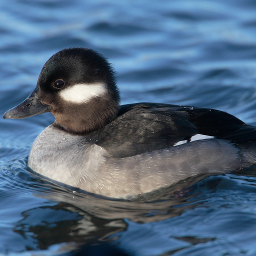
\includegraphics[width=\textwidth]{img/fca/duck1}
    \\ \color{green}{\footnotesize $hasBill(x) \wedge isDuck(x)$}
  \end{minipage}
  \hfill
  \begin{minipage}[t]{0.3\linewidth}
    \vspace{0pt}
    \centering
    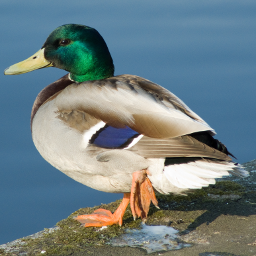
\includegraphics[width=\textwidth]{img/fca/duck2}
    \\ \color{green}{\footnotesize $hasBill(y) \wedge isDuck(y)$}
  \end{minipage}
  \hfill
  \pause
  \begin{minipage}[t]{0.3\linewidth}
    \vspace{0pt}
    \centering
    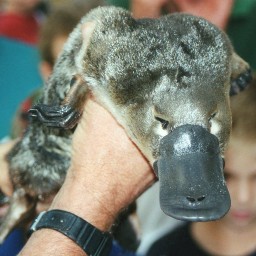
\includegraphics[width=\textwidth]{img/fca/platypus}
    \\ \color{red}{\footnotesize $hasBill(z) \wedge \neg{}isDuck(z)$}
  \end{minipage}
\end{figure}

\end{frame}

%-------------------------------------------------------------------------------
% FASTER QUERIES
%
%% on peut en dégager une hiérarchie des RPBS. Celle-ci pourrait
%% permettre une recherche plus intelligente des RPBS (réduction du
%% nombre d'homomorphismes à appliquer sur chaque plateau) et donc un
%% gain de temps pour la prise de décision sans devoir réduire
%% drastiquement le nombre de RPBS. On peut imaginer que le système
%% effectuerait une recherche approfondie à posteriori afin de ne pas
%% biaiser l'apprentissage. (L'idée générale est, pendant la phase de
%% jeu, de classer le CBS à évaluer dans un concept et de lui
%% attribuer le point associé à celui-ci. Ce qui permettrait de
%% profiter de la structure du treillis pour diminuer drastiquement le
%% nombre de RPBS rechercher. À savoir que c'est l'étape la plus
%% coûteuse.)
%-------------------------------------------------------------------------------
\subsection{Faster queries}
\begin{frame}{What FCA brings to the table}{Faster queries}


  \begin{itemize}
    \item Le treillis de FCA nous offre un ordre partiel sur les
      configurations de plateau
    \item Il est possible de ce servir de cette ordre pour effectuer
      une exploration partiel des configurations lors de l'analyse
      d'un plateau
    \item toutefois pour ne pas biaiser cette ordre partiel il est
      important d'effectuer une recherche complète a posteriori
    
  \end{itemize}



\end{frame}

%-------------------------------------------------------------------------------
% CHOOSING NEW CONFIGURATIONS 
%
%% Les RPBS introduit dans des concepts
%% parents d'un concept commun (introduisant au moins un CBS), ont
%% potentiellement une sous-partie commune qu'il peut-être intéressant
%% d'extraire comme un nouveau RPBS. (voir common_part.png)
% -------------------------------------------------------------------------------
\subsection{Discovering new configurations}
\begin{frame}{What FCA brings to the table}{Discovering new
    configurations}

\begin{minipage}[t]{0.40\linewidth}
  \begin{figure}[ht]
    \centering
    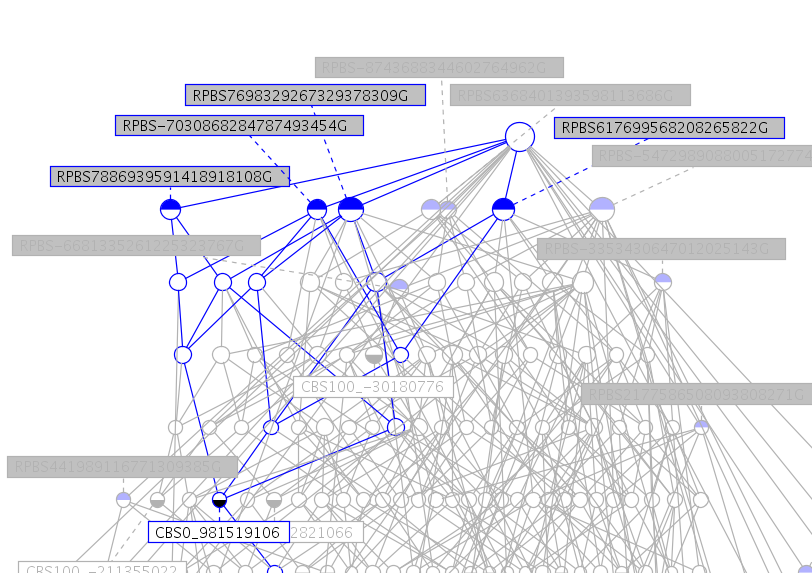
\includegraphics[width=\textwidth]{img/fca/common_part}
  \end{figure}
\end{minipage}
\begin{minipage}{0.50\linewidth}
  \begin{figure}[ht]
    \centering
    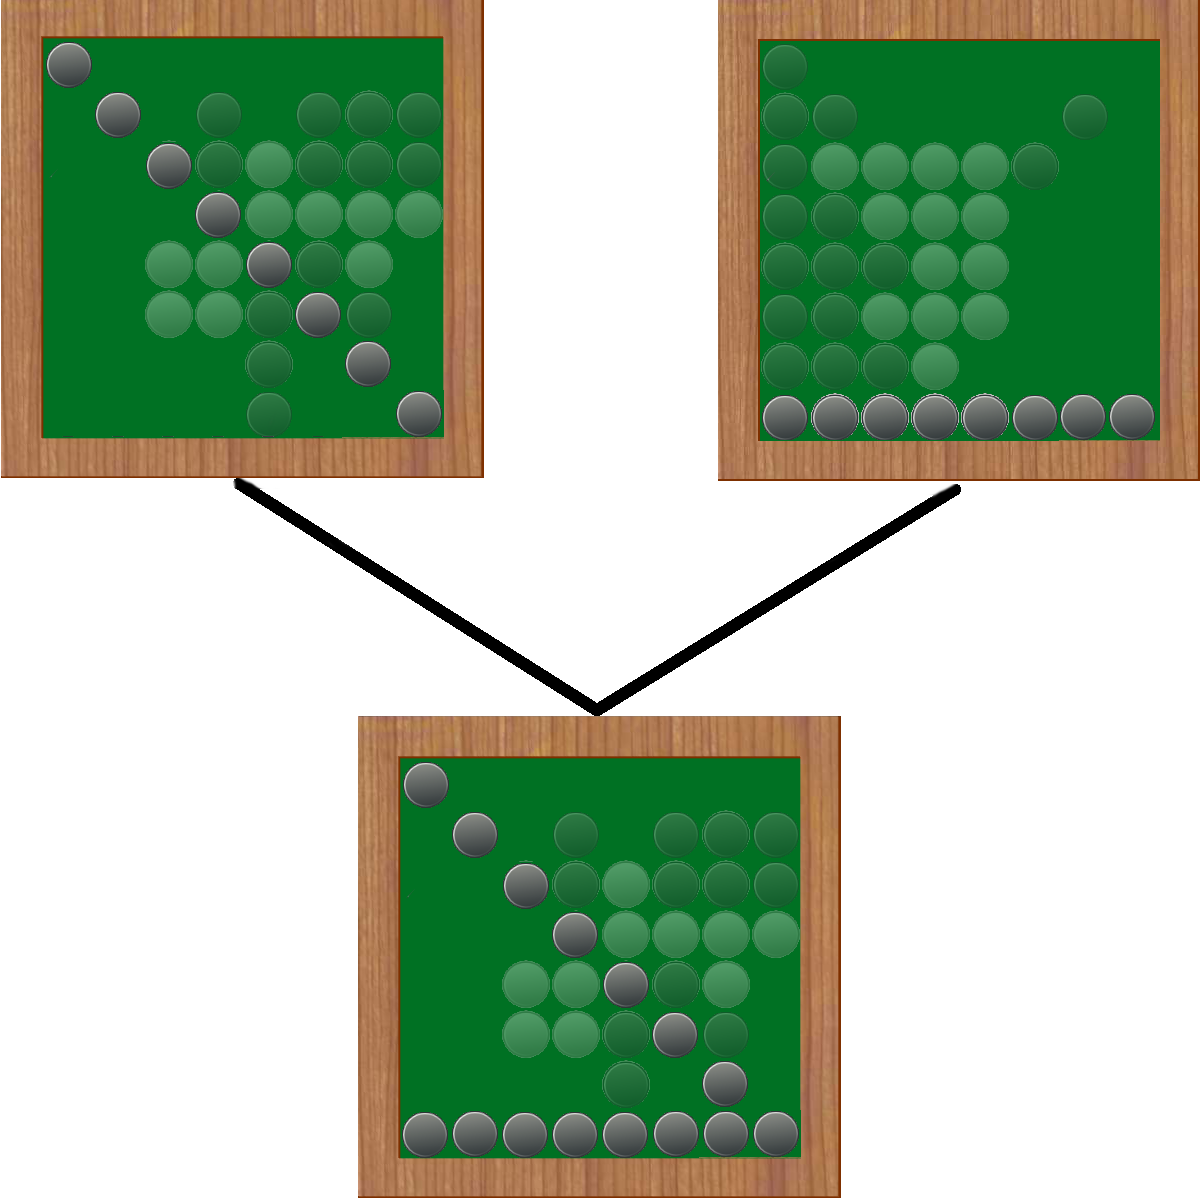
\includegraphics[width=\textwidth]{img/fca/fca_new_configuration}
  \end{figure}  

\end{minipage}

\end{frame}


% ADDED INSIGHT
%-------------------------------------------------------------------------------
\subsection{Added insight}
\begin{frame}{What FCA brings to the table}{Added insight}

\begin{minipage}[t]{0.40\linewidth}
  \begin{figure}[ht]
    \centering
    %\includegraphics[width=\textwidth]{}
  \end{figure}
\end{minipage}
\begin{minipage}{0.59\linewidth}
  \begin{itemize}
    \item 
  \end{itemize}
\end{minipage}

\end{frame}